\documentclass{beamer}

\usepackage[english]{babel}
\usepackage[utf8]{inputenc}
\usepackage{hyperref}
\usepackage{amsmath}
\usepackage{amssymb}

\usepackage{tikz}
\usepackage{subfigure}

\usepackage{comment}

\newcommand{\todo}[1]{\textcolor{red}{TODO: #1}}
\newcommand{\korrektur}[1]{\textcolor{red}{\textbf{Korrektur:} #1}}
\newcommand{\reals}{\mathbb{R}}

\newcommand{\zoomfactor}{0.6}
\newcommand{\autozoomfactor}{0.15}

\renewcommand{\zoomfactor}{0.3}
\renewcommand{\autozoomfactor}{0.075}

\title{Comparing polynomials arising from exact and approximate solution of the Lax-Friedrich-Flux}
\author{Stjepan Bakrac \and Philipp Müller}
\date{}

\newcommand{\partialderivative}[1]{\dfrac{\partial}{\partial #1}}
\newcommand{\pd}[2]{\dfrac{\partial #1}{\partial #2}}
\newcommand{\totalderivative}[1]{\dfrac{d}{d #1}}
\newcommand{\naturals}{\mathbb{N}}

\renewcommand{\phi}{\varphi}

\newcommand\intend{\mathrm{d}}

\DeclareMathOperator{\divergence}{div}

\AtBeginPart{\frame{\partpage}}

\begin{document}

\part{Derivation of stuff.}
\label{part:introduction}

\begin{frame}
  \frametitle{Introduction}
  \begin{itemize}
  \item Wave simulation
  \item (Adaptive) triangulation of the whole area
  \item How can we model the flux between triangles?
  \item Model continuous equations within these triangles
  \end{itemize}
\end{frame}

\section{Discontinuous Galerkin Method}
\label{sec:basis-functions-intro}

\begin{frame}
  \frametitle{Shallow Water Equations}
  \begin{equation}
    \label{eq:shallow-water-raw}
    \pd{\mathbf{q}}{t} + \divergence F(\mathbf{q}) = r = \begin{pmatrix}
      0 \\ 0\\ 0
    \end{pmatrix}
  \end{equation}

  \begin{block}{Two variants for $F$:}
    \begin{eqnarray*}
      \mathbf{q} =
      \begin{pmatrix}
        h \\ h v_x \\ h v_y
      \end{pmatrix} \quad F(\mathbf{q}) =
      \begin{pmatrix}
        h \mathbf{v} \\ h v_x \mathbf{v} + \frac{1}{2} g h^2 e_x \\ h
        v_y \mathbf{v} + \frac{1}{2} g h^2 e_y
      \end{pmatrix}
    \end{eqnarray*}

    \begin{eqnarray*}
      \mathbf{q} =
      \begin{pmatrix}
        h \\ u_x \\ u_y
      \end{pmatrix} \quad F(\mathbf{q}) =
      \begin{pmatrix}
        \mathbf{u} \\ \frac{u_x}{h} \mathbf{u} + \frac{1}{2} g h^2 e_x \\ \frac{u_y}{h} \mathbf{u}+
        \frac{1}{2} g h^2 e_y
      \end{pmatrix},
    \end{eqnarray*}
    where $\mathbf{u}=
    \begin{pmatrix}
      u_x \\ u_y
    \end{pmatrix}$ and $\mathbf{v} =
    \begin{pmatrix}
      v_x \\ v_y
    \end{pmatrix}$
  \end{block}
\end{frame}

\begin{frame}
  \frametitle{$x$- and $y$-Direction}

  \begin{equation*}
    \pd{\mathbf{q}}{t} + \divergence F(\mathbf{q}) = r = \begin{pmatrix}
      0 \\ 0\\ 0
    \end{pmatrix}
  \end{equation*}

  \begin{eqnarray*}
    \mathbf{q} =
    \begin{pmatrix}
      h \\ u_x \\ u_y
    \end{pmatrix} \quad F(\mathbf{q}) =
    \begin{pmatrix}
      u \\ \frac{u_x}{h} \mathbf{u} + \frac{1}{2} g h^2 e_x \\ \frac{u_y}{h} \mathbf{u} +
      \frac{1}{2} g h^2 e_y
    \end{pmatrix}
  \end{eqnarray*}

  \begin{eqnarray*}
    F^x(\mathbf{q}) =
    \begin{pmatrix}
      u_x \\ \frac{u_x^2}{h} + \frac{1}{2} g h^2 \\ \frac{u_x u_y}{h}
    \end{pmatrix}
    \quad
    F^y(\mathbf{q}) =
    \begin{pmatrix}
      u_y \\ \frac{u_x u_y}{h} \\ \frac{u_y^2}{h} + \frac{1}{2} g h^2
    \end{pmatrix}
  \end{eqnarray*}
  
  \begin{block}{Remarks:}
    \begin{itemize}
    \item Difference between $\mathbf{q}$ and $u=(u_x,u_y)$.
    \item Each line consists of 2 sub-lines ($x$- and $y$-direction).
    \item $\divergence
      \begin{pmatrix}
        a \\ b
      \end{pmatrix} = \pd{a}{x} + \pd{b}{y}$
    \end{itemize}
  \end{block}
  \todo{Erklären, dass man durch $\divergence$ insgesamt 3 Zeilen enthält.}
  
\end{frame}

\begin{frame}
  \frametitle{Weak Form}
  \begin{equation}
    \label{eq:shallow-water-weak-form}
    \int_T \pd {\mathbf{q}}{t} \phi \, dT + \int_T \nabla \cdot F(\mathbf{q}) \phi \, dT = 0
  \end{equation}
  
  \begin{block}{Remarks:}
    \begin{itemize}
    \item Galerkin method: Multiply equation (\ref{eq:shallow-water-raw}) by $\phi$ and integrate over triangle $T$
    \item Integral works line by line (i.e. for components $h$, $u_x$ and $u_y$)
    \item $\nabla \cdot F(\mathbf{q}) = \divergence F(\mathbf{q})$
    %\item $T$ is a single triangle
    \end{itemize}
  \end{block}
  \todo{Erklärung von Stjepan bezgl. Dreiecke auch in Slides bringen!}

  Gaussian Divergence Theorem yields:
  \begin{equation*}
    \int_T \pd {\mathbf{q}}{t} \phi \, dT +
    \int_{\partial T} F(\mathbf{q}) \cdot n \phi \, ds -
    \int_T F(\mathbf{q}) \cdot \nabla \phi \, dT = 0
  \end{equation*}

\end{frame}

\begin{frame}
  \frametitle{Weak Form -- Some Explanations}
  \begin{equation}
    \label{eq:shallow-water-weak-form-div-applied}
    \int_T \pd {\mathbf{q}}{t} \phi \, dT +
    \int_{\partial T} F(\mathbf{q}) \cdot n \phi \, ds -
    \int_T F(\mathbf{q}) \cdot \nabla \phi \, dT = 0
  \end{equation}
  
  \begin{block}{Remarks:}
    \begin{itemize}
    \item $dT$ and $ds$: abbreviations for $dx\ dy$
    %\item First integral: Straightforward!
    \item Second integral:
      \begin{itemize}
      \item Border integral ``around'' triangle
      \item $n$ denotes the normal (depending upon $x,y$-values)
      \end{itemize}
    \item Third integral: $\nabla
      \begin{pmatrix}
        a \\ b
      \end{pmatrix} =\left( \pd{a}{x}, \pd{b}{y} \right) ^T$
    \item ``Multiplications'': $(a,b)\cdot(c,d) = ac+bd$
    \item Goal: Find solution for $\mathbf{q}$
    \end{itemize}
  \end{block}
\end{frame}

\begin{frame}
  \frametitle{Galerkin Method}
  \begin{itemize}
  \item Have several functions $\phi_i$ (for $i=1:n$) -- will be defined later
  \item Approximation: 
    $\mathbf{q} \approx \sum_{i=1}^n \mathbf{q}_i \phi_i(x,y)$.
  \item Only $\phi_i$ depending on $x,y$!
  \end{itemize}

  \begin{equation}
    \label{eq:shallow-water-weak-form-div-applied-approximation}
    \int_T \pd {\mathbf{q}}{t} \phi_i \, dT +
    \sum_{e\in\left\{ e_1,e_2,e_3 \right\}} \int_{e} F^e \phi_i \, ds  -
    \int_T F(\mathbf{q}) \cdot \nabla \phi_i \, dT = 0
  \end{equation}
\end{frame}

\section{Matrices, matrices, matrices}

\begin{frame}
  \frametitle{First Integral: Mass Matrix}

  \begin{eqnarray*}
    \int_T \pd {\mathbf{q}}{t} \phi_i \, dT &\approx& 
    \int_T \pd {\left( \sum_{j=1}^n \mathbf{q}_j \phi_j \right) }{t} \phi_i \, dT = \\
    &=& \sum_{j=1}^n \underbrace{\int_T \phi_i \phi_j \, dT}_{M_{ij}} \pd{\mathbf{q}_j}{t}
  \end{eqnarray*}
  
  \begin{block}{}
    \begin{itemize}
    \item Symmetric $n \times n$-matrix
    \item Interpret the above as a matrix multiplication
    \end{itemize}
  \end{block}

  \begin{equation*}
    \int_T \pd {\mathbf{q}}{t} \phi_i \, dT \approx
    M \cdot \pd{
        \left( \mathbf{q}_1 , \dots , \mathbf{q}_n  \right)^T }
      {t}
  \end{equation*}
\end{frame}

\begin{frame}
  \frametitle{Third Integral: Stiffness matrix -- $h$-component}
  \begin{eqnarray*}
    \int_T F_1(\mathbf{q}) \cdot \nabla \phi_i \, dT &=&
    \int_T
    \begin{pmatrix}
      u_x \\ u_y
    \end{pmatrix}
    \cdot \nabla \phi_i \, dT \approx \\
    &=& \int_T 
    \begin{pmatrix} 
      \sum_{j=1}^n u_{x,j} \phi_j \\
      \sum_{j=1}^n u_{y,j} \phi_j \\
    \end{pmatrix}
    \cdot 
    {
      \renewcommand\arraystretch{2}
      \begin{pmatrix}
        \pd{\phi_i}{x} \\
        \pd{\phi_i}{y} 
      \end{pmatrix} dT 
    }\\
    &=& \sum_{j=1}^n u_{x,j} \underbrace{\int_T \phi_j \pd{\phi_i}{x} \, dT}_{S^x_{ij}} + \sum_{j=1}^n u_{y,j} \underbrace{\int_T \phi_j \pd{\phi_i}{y} \, dT}_{S^y_{ij}}
  \end{eqnarray*}
  \begin{block}{}
    \begin{itemize}
    \item $S^x$ and $S^y$ are $n \times n$-matrices
    \item Interpret sums as matrix multiplications
    \end{itemize}
  \end{block}
\end{frame}

\begin{frame}
  \frametitle{Intermezzo: Point-wise Approximation}
  \begin{itemize}
  \item   $\mathbf{q}\approx \sum_{i=1}^n \mathbf{q}_i \phi_i$, i.e.\,$
    \begin{pmatrix}
      h \\ u_x \\ u_y
    \end{pmatrix} = \sum_{i=1}^n
    \begin{pmatrix}
      h_i \\ u_{x,i} \\ u_{y,i}
    \end{pmatrix}
    \phi_i$
  \item   We would like to compute function value
    \begin{equation*}
      f(\mathbf{q}) \approx 
      f\left(\sum_{i=1}^n h_i \phi_i,
        \sum_{i=1}^n u_{x,i} \phi_i,
        \sum_{i=1}^n u_{y,i} \phi_i\right),
    \end{equation*}
  \item   Too complex $\Rightarrow$ compute the following:
    \begin{equation*}
      \sum_{i=1}^n f(h_i,u_{x,i},u_{y,i}) \phi_i.
    \end{equation*}
  \end{itemize}
\end{frame}

\begin{frame}
  \frametitle{Third Integral: Stiffness matrix -- $u_x$-component}
  \begin{eqnarray*}
    \label{sec:third-integral-second-line-1}
    \int_T F_2(\mathbf{q}) \cdot \nabla \phi_i \, dT &=&
    \int_T
    \begin{pmatrix}
      \frac{u_x^2}{h} + \frac{1}{2} g h^2 \\ \frac{u_x u_y}{h}
    \end{pmatrix}
    \cdot \nabla \phi_i \, dT \approx \\        
    \label{sec:third-integral-second-line-2}
    &=& 
    \int_T 
    \begin{pmatrix}
      \sum_{j=1}^n \left(\frac{u_{x,j}^2}{h_j^2} + \frac{1}{2} g h_j^2\right) \phi_j \\
      \sum_{j=1}^n \left(\frac{u_{x,j} u_{y,j}}{h_j}\right) \phi_j \\
    \end{pmatrix}
    \cdot 
    \begin{pmatrix}
      \pd{\phi_i}{x} \\
      \pd{\phi_i}{y} 
    \end{pmatrix} dT \\
    &=& \nonumber \sum_{j=1}^n \left(\frac{u_{x,j}^2}{h_j^2} + \frac{1}{2} g h_j^2\right) \int_T \phi_j \pd{\phi_i}{x} \, dT \\ 
    &&+ \nonumber \sum_{j=1}^n \left(\frac{u_{x,j} u_{y,j}}{h_j}\right) \int_T \phi_j \pd{\phi_i}{y} \, dT
  \end{eqnarray*}
    \begin{itemize}
    \item First to second line uses a point-wise approximation
    \item We recognize the stiffness matrices $\Rightarrow$ interpret as matrix multiplication
    \end{itemize}
\end{frame}

\begin{frame}
  \frametitle{Third Integral: Stiffness matrix -- $u_y$-component}
  \begin{eqnarray*}
    \int_T F_3\left(\mathbf{q}\right) \cdot \nabla \phi_i \, dT &=&
    \int_T
    \begin{pmatrix}
      \frac{u_x u_y}{h} \\ \frac{u_y^2}{h} + \frac{1}{2} g h^2 
    \end{pmatrix}
    \cdot \nabla \phi_i \, dT \approx \\
    &=& \int_T 
    \begin{pmatrix}
      \sum_{j=1}^n \left(\frac{u_{x,j} u_{y,j}}{h_j}\right) \phi_j \\
      \sum_{j=1}^n \left(\frac{u_{y,j}^2}{h_j^2} + \frac{1}{2} g h_j^2\right) \phi_j \\
    \end{pmatrix}
    \cdot 
    \begin{pmatrix}
      \pd{\phi_i}{x} \\
      \pd{\phi_i}{y} 
    \end{pmatrix} dT \\
    &=& \sum_{j=1}^n \left(\frac{u_{x,j} u_{y,j}}{h_j}\right) \int_T \phi_j \pd{\phi_i}{x} \, dT \\
    &&+ \sum_{j=1}^n \left(\frac{u_{y,j}^2}{h_j^2} + \frac{1}{2} g h_j^2\right) \int_T \phi_j \pd{\phi_i}{y} \, dT
  \end{eqnarray*}

\end{frame}

\begin{frame}
  \frametitle{Second Integral}
  Split into triangle edges:
  \begin{equation}
    \label{eq:border-integral-sum}
    \int_{\partial T} F(\mathbf{q}) \cdot n \phi_i \, ds = \sum_{e\in\left\{ e_1,e_2,e_3 \right\}} \int_{e} F^e \phi_i \, ds =: BI
  \end{equation}
  \begin{itemize}
  \item Normals are incorporated in $F^e$
  \end{itemize}
\end{frame}

\begin{frame}
    \frametitle{Border Integral}
    Compute $\sum_{e\in\left\{ e_1,e_2,e_3 \right\}} \int_{e} F^e \phi_i \, ds$ by Gauss-Quadrature:

\begin{equation}
  \int_{e} F^e \phi_i \, ds \approx \sum_{k=0}^{m} F^e(p_k) \underbrace{\phi_i(p_k) \cdot w_k}_{W_{ik}},
\end{equation}
\todo{Sollte das $F^e_j$ heißen?}
\begin{block}{Remarks}
  \begin{itemize}
  \item $m$: Number of support points for Gaussian quadrature
  \item $p_k$: Gauss-support point with index $k$
  \item $w_k$: corresponding Gauss weight
  \item $W_{ik}$: $n\times m$ matrix; can be pre-computed!
  \item $F^e$: Numerical flux (several possibilities)
  \end{itemize}
\end{block}
    
\end{frame}

\begin{frame}
  \frametitle{Overview: Matrices}
  \begin{description}
  \item[Mass matrix.] The mass matrix is a $(n\times n)$-matrix that has the following structure:
    \begin{equation}
      \label{eq:mass-matrix-overview}
      M_{ij} = \int_T \phi_i \phi_j \ dT
    \end{equation}
  \item[Stiffness matrices] Stiffness matrices have dimension $(n\times n)$. They are computed as follows:
    \begin{equation}
      \label{eq:stiffness-matrix-overview}
      S^x_{ij} = \int_T \phi_j \pd{\phi_i}{x} \quad
      S^y_{ij} = \int_T \phi_j \pd{\phi_i}{y}
    \end{equation}
  \item[``Weight matrix''] This matrix has dimensions $n\times m$, and is computed as follows:
    \begin{equation}
      \label{eq:edge-matrix}
      W_{ik} = \phi_i(p_k)\cdot w_k
    \end{equation}
  \end{description}
\end{frame}

\begin{frame}
  \frametitle{Rewriting Equations}
  Remember:
  \begin{equation*}
    \int_T \pd {\mathbf{q}}{t} \phi \, dT +
    \int_{\partial T} F(\mathbf{q}) \cdot n \phi \, ds -
    \int_T F(\mathbf{q}) \cdot \nabla \phi \, dT = 0
  \end{equation*}
  Using matrices $\tilde{\mathbf{q}} = (\mathbf{q}_1,\dots,\mathbf{q}_n)$ and $\tilde{F^e}=(F^e(p_1),\dots,F^e(p_n))$, \todo{Stimmt die Definition von $\tilde{F^e}$?}we can rewrite:
  
  \begin{equation*}
    M \cdot \pd{\tilde{\mathbf{q}}}{t} +
    \sum_{e \in E} \tilde{F^e} W -
    \left(F^x(\tilde{\mathbf{q}}) \cdot S^x +
      F^y(\tilde{\mathbf{q}}) \cdot S^y\right) = 0
  \end{equation*}
\end{frame}

\begin{frame}
  \frametitle{Choice of Basis Functions $\phi_i$}
  \begin{itemize}
  \item Polynomial basis functions (in two variables $x$ and $y$)
  \item Basis function have to \emph{span} space of all polynomials up to a certain degree
  \end{itemize}
  Simple way:
  \begin{itemize}
  \item Grab a certain set of $n$ points $p_1$ through $p_{n}$.
  \item Construct basis function $\phi_i$ such that $\forall i=1:n \  \forall j=1:n. \ \phi_i(p_j) = \delta_{ij}$ using lagrange polynomials (the term $\delta_{ij}$ denotes Kronecker-Delta).
  \end{itemize}
  Consequences:
  \begin{itemize}
  \item Polynomials of degree $d$ $\Rightarrow$ $\binom{d+2}{2}$ basis functions resp. support points
  \end{itemize}
\end{frame}

\begin{frame}
  \frametitle{Support Points}
  \begin{itemize}
  \item Low degree of basis function: Specific support points
    \begin{itemize}
    \item 0: Support point in center of triangle
    \item 1: 3 points at the centers of the edges
    \item 2: 6 points: center of edges and triangle corners
    \end{itemize}
  \item Higher degree: ``Dunavant-Method'' \todo{Genauer erklären?}\todo{Referenz.}
  \end{itemize}

\begin{figure}[ht]
  \centering
  \subfigure[Degree 0]{
    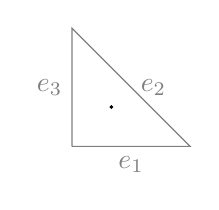
\begin{tikzpicture}[scale=1.5]
      \draw[opacity=0.5] (0,0) -- node[left]{$e_3$} (0,1) -- node[right]{$e_2$} (1,0) -- node[below]{$e_1$} (0,0);
      \draw[fill=black] (0.33333333, 0.3333333333) circle (0.01);
    \end{tikzpicture}
  }
  \subfigure[Degree 1]{
    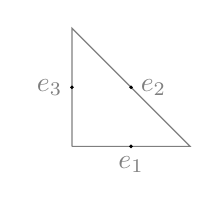
\begin{tikzpicture}[scale=1.5]
      \draw[opacity=0.5] (0,0) -- node[left]{$e_3$} (0,1) -- node[right]{$e_2$} (1,0) -- node[below]{$e_1$} (0,0);
      \draw[fill=black] (0.5, 0) circle (0.01);
      \draw[fill=black] (0, 0.5) circle (0.01);
      \draw[fill=black] (0.5, 0.5) circle (0.01);
    \end{tikzpicture}
  }
  \subfigure[Degree 2]{
    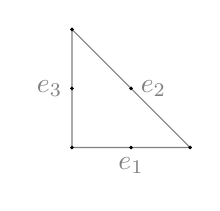
\begin{tikzpicture}[scale=1.5]
      \draw[opacity=0.5] (0,0) -- node[left]{$e_3$} (0,1) -- node[right]{$e_2$} (1,0) -- node[below]{$e_1$} (0,0);
      \draw[fill=black] (0.5, 0) circle (0.01);
      \draw[fill=black] (0, 0.5) circle (0.01);
      \draw[fill=black] (0.5, 0.5) circle (0.01);
      \draw[fill=black] (0, 0) circle (0.01);
      \draw[fill=black] (1, 0) circle (0.01);
      \draw[fill=black] (0, 1) circle (0.01);
    \end{tikzpicture}
  }
  \subfigure[Degree 3]{
    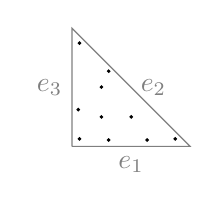
\begin{tikzpicture}[scale=1.5]
      \draw[opacity=0.5] (0,0) -- node[left]{$e_3$} (0,1) -- node[right]{$e_2$} (1,0) -- node[below]{$e_1$} (0,0);
      \draw[fill=black] (0.501426509658179, 0.24928674517091) circle (0.01);
      \draw[fill=black] (0.24928674517091, 0.24928674517091) circle (0.01);
      \draw[fill=black] (0.24928674517091, 0.501426509658179) circle (0.01);
      \draw[fill=black] (0.873821971016996, 0.063089014491502) circle (0.01);
      \draw[fill=black] (0.063089014491502, 0.063089014491502) circle (0.01);
      \draw[fill=black] (0.063089014491502, 0.873821971016996) circle (0.01);
      \draw[fill=black] (0.053145049844817, 0.310352451033784) circle (0.01);
      \draw[fill=black] (0.310352451033784, 0.636502499121399) circle (0.01);
      \draw[fill=black] (0.636502499121399, 0.053145049844817) circle (0.01);
      \draw[fill=black] (0.310352451033784, 0.053145049844817) circle (0.01);
    \end{tikzpicture}
  }
\end{figure}

\end{frame}

\begin{frame}
  \frametitle{Intermezzo: Explicit Euler}
\begin{eqnarray}
  \label{eq:euler-method-setting}
  \pd{x(t)}{t} &=& f(t, x(t)). \\
  x(t_0) &=& x_0
\end{eqnarray}

Timesteps with distance $\tau$: $t_{k+1} = t_k + \tau$.

\begin{equation}
  \label{eq:euler-step-solution}
  x_{k+1} = x_k + \tau f(t_k, x_k), \quad k=0,1,2,\dots
\end{equation}

\end{frame}

\begin{frame}
  \frametitle{Solving the Equation}
  \begin{equation*}
    M \cdot \pd{\tilde{\mathbf{q}}}{t} +
    \sum_{e \in E} \tilde{F^e} W -
    \left(F^x(\tilde{\mathbf{q}}) \cdot S^x +
      F^y(\tilde{\mathbf{q}}) \cdot S^y\right) = 0
  \end{equation*}
  Rearrange and left-multiply with $M^{-1}$, afterwards Euler:
  \begin{equation*}
    \pd{\tilde{\mathbf{q}}}{t} =
    M^{-1} \cdot \left(
      F^x(\tilde{\mathbf{q}}) \cdot S^x +
      F^y(\tilde{\mathbf{q}}) \cdot S^y -
      \sum_{e \in E} \tilde{F^e} W\right
    )
  \end{equation*}
  \begin{equation*}
    \Rightarrow \quad
    \tilde{\mathbf{q}}_{k+1} =
    \tilde{\mathbf{q}}_{k} +
    \tau \cdot M^{-1} \cdot \left(
      F^x(\tilde{\mathbf{q}}) \cdot S^x +
      F^y(\tilde{\mathbf{q}}) \cdot S^y -
      \sum_{e \in E} \tilde{F^e} W\right
    ),
  \end{equation*}
  where $\tilde{\mathbf{q}} = (\mathbf{q}_1,\dots,\mathbf{q}_n)$ and $\tilde{\mathbf{q}}_k$ is the value of $\tilde{\mathbf{q}}$ at time $k$.

  \begin{block}{Remark}
    Actually a collection of $3n$ equations!
  \end{block}
\end{frame}

\part{Comparing polynomials arising from exact and approximate solution of the Lax-Friedrich-Flux}
\label{part:polynomialstuff}

\begin{frame}
  \frametitle{Flux Function and Lax-Friedrich-Flux}
  Flux:
  \begin{equation}
    \label{eq:flux-function-definition}
    F\left(
      \begin{pmatrix}
        h \\ u
      \end{pmatrix}
    \right) = 
    \begin{pmatrix}
      u \cdot h \\
      \frac{1}{2} g h^2 + u^2 \cdot h
    \end{pmatrix}
  \end{equation}
  Lax-Friedrich:
  \begin{equation}
    \label{eq:lax-friedrich-definition}
    F_{LF}(p^R,p^L) = \dfrac{1}{2}\cdot (F(p^R) + F(p^L)) - \alpha \cdot (p^R - p^L)
  \end{equation}
  \begin{block}{Remarks:}
    \begin{itemize}
    \item $p^R, p^L$: Data from the right and left triangle, respectively, containing height and impulse ($h$ and $u$)
    \item $p^R, p^L$ can be fix over the whole triangle or can be functions (e.g. polynomials) returning two components
    \end{itemize}
  \end{block}
\end{frame}

\begin{frame}
  \frametitle{Original Situation: 2d-Problem}
  \begin{center}
    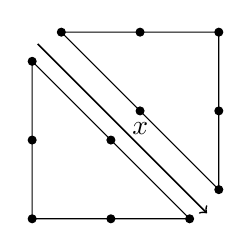
\begin{tikzpicture}[scale=2]
      \begin{scope}[xshift=-.1em,yshift=-.1em]
        \draw (0,0) -- (0,1) -- (1,0) -- (0,0); \draw[fill=black]
        (0,0) circle (0.025); \draw[fill=black] (0.5,0) circle
        (0.025); \draw[fill=black] (1,0) circle (0.025);
        \draw[fill=black] (0.5,0.5) circle (0.025); \draw[fill=black]
        (0,1) circle (0.025); \draw[fill=black] (0,0.5) circle
        (0.025);
      \end{scope}
      \draw[->,semithick] (0,1.075) -- node[right]{$x$} (1.075,0);
      \begin{scope}[xshift=1.15cm,yshift=1.15cm,rotate=180]
        \draw (0,0) -- (0,1) -- (1,0) -- (0,0); \draw[fill=black]
        (0,0) circle (0.025); \draw[fill=black] (0.5,0) circle
        (0.025); \draw[fill=black] (1,0) circle (0.025);
        \draw[fill=black] (0.5,0.5) circle (0.025); \draw[fill=black]
        (0,1) circle (0.025); \draw[fill=black] (0,0.5) circle
        (0.025);
      \end{scope}
    \end{tikzpicture}
  \end{center}
  \begin{itemize}
  \item Two adjacent triangles
  \item Height and impulse is an own polynomial function for \emph{each} triangle $\Rightarrow$ Discontinuity along the common edge
  \item We are interested in the situation along the common edge
  \item Parametrize edge, such that we can choose $x\in \left[ 0,1 \right]$ and ``obtain everything just depending upon this single variable''
  \end{itemize}

\end{frame}

\begin{frame}
  \frametitle{Constructing the Polynomials}
  Remember:
  \begin{equation*}
    F_{LF}(p^R,p^L) = \dfrac{1}{2}\cdot (F(p^R) + F(p^L)) - \alpha \cdot (p^R - p^L)
  \end{equation*}
  \begin{itemize}
  \item Pick $n$ points for each of the edges: Points of the left triangle:
    $\left(x_1,\begin{pmatrix}
        h_1^R \\ u_1^R
      \end{pmatrix}\right), \dots , \left(x_n, \begin{pmatrix}
        h_n^R \\ u_n^R
      \end{pmatrix}\right)$ and the points for the right triangle 
    $\left(x_1,\begin{pmatrix}
        h_1^L \\ u_1^L
      \end{pmatrix}\right), \dots , \left(x_n,\begin{pmatrix}
        h_n^L \\ u_n^L
      \end{pmatrix}\right)$.
  \item Assign height and impulse to each of the $2n$ points
  \item Generate 4 polynomials by interpolation
    \begin{itemize}
    \item Height, right triangle: $(x_i, h_i^R)$
    \item Impulse, right triangle: $(x_i, u_i^R)$
    \item Height, left triangle: $(x_i, h_i^L)$
    \item Impulse, left triangle: $(x_i, u_i^L)$
    \end{itemize}
  \item Group right polynomials into $p^R$, left polynomials into $p^L$
  \end{itemize}
\end{frame}

\begin{frame}
  \frametitle{Choice of Support Points for Polynomials}
  \begin{itemize}
  \item In principle: arbitrary
  \item In practice: Use support points from Gaussian quadrature since we'll apply it later
  \item We also tested equidistant support points
  \end{itemize}
  \todo{Bild von support points auf Kante einfügen.}
\end{frame}

\begin{frame}
  \frametitle{Interpolation}
  Interpolation routine:
  \begin{equation*}
    interpolate(\{(x_i,y_i) \mid i \in \{1 \dots n\}\})
  \end{equation*}
  yields a polynomial of minimum degree (i.e. $n-1$) interpolating all given points $(x_i,y_i)$.

  Shorter notation: 
  \begin{equation*}
    interpolate(x,y)
  \end{equation*}

  \begin{itemize}
  \item $p^L_h(x) := interpolate (x,h^L)$. Height for left triangle.
  \item $p^L_u(x) := interpolate (x,u^L)$. Impulse for left triangle.
  \item $p^R_h(x) := interpolate (x,h^R)$. Height for right triangle.
  \item $p^R_u(x) := interpolate (x,u^L)$. Impulse for right triangle.
  \end{itemize}

  \begin{equation*}
    p^L(x) :=
    \begin{pmatrix}
      p^L_h(x) \\ p^L_u(x)
    \end{pmatrix}, \quad
    p^R(x) :=
    \begin{pmatrix}
      p^R_h(x) \\ p^R_u(x)
    \end{pmatrix}
  \end{equation*}
\end{frame}

\begin{frame}
  \frametitle{Goal}
  \begin{block}{Comparison of $N(x)$ and $N'(x)$}
    \begin{description}
    \item[Exact solution] $N(x) := F_{LF}(p^R(x),p^L(x))$
    \item[Approximate solution] \todo{Hier stimmts im Skript noch nicht! Das muss $y_i^F$ heißen.}
      \begin{equation*}
        F_{LF}\left(
          \begin{pmatrix}
            h_i^R \\ u_i^R
          \end{pmatrix},
          \begin{pmatrix}
            h_i^L \\ u_i^L
          \end{pmatrix}
        \right) :=
        \begin{pmatrix}
          h_i^F \\ u_i^F
        \end{pmatrix} = y_i^F
      \end{equation*}

      \begin{equation*}
        N'(x) :=
        \begin{pmatrix}
          interpolate(x,h^F) \\ interpolate(x,u^F)
        \end{pmatrix}
      \end{equation*}
    \end{description}
  \end{block}
  $\Rightarrow$ Comparison by 
  $I := \int\limits_{x=0}^1 | N(x) - N'(x) |\  dx$

\end{frame}

\begin{frame}
  \frametitle{Evaluating $I$}
  \begin{itemize}
  \item Complicated analycital solution (absolute value/rational function)
  \item Possibility 1: Approximate $I$ by $\int\limits_{x=0}^1 N(x) - N'(x) \  dx$
    \begin{itemize}
    \item Not good.
    \end{itemize}
  \item Fact: $N(x_i) = N'(x_i)$ 
    $\Rightarrow$ $N(x_i) - N'(x_i) = 0$
  \item Piecewise integration between the $x_i$'s: \todo{Sollten im Skript die Betragsstriche nicht anders stehen (so wie hier)?}
    \begin{equation*}
      \sum\limits_{i=1}^{n-1} \left|\ \int\limits_{x=x_i}^{x_{i+1}} N(x) - N'(x) \  dx\ \right|
    \end{equation*}
    \begin{itemize}
    \item Seems quite good, but really, really, really slow
    \item Accuracy can be improved by ``adding $x_i$'s''
    \end{itemize}
  \end{itemize}
\end{frame}

\begin{frame}
  \frametitle{Evaluating $I$ -- Numerical integration}
  \begin{itemize}
  \item Maple's intrinsic integration:  
    \begin{center}
      \texttt{evalf(Int(abs(N(x)-N'(x)),x=0..1))}
    \end{center}
    works, but takes much too long for general parameters!
  \item Old-school: Numerical integration using the ``Streifenmethode'' \todo{Wie heißt das auf Englisch?} \todo{Im Skript diese Methode nachreichen!}
  \end{itemize}
\end{frame}

\begin{frame}
  \frametitle{Some Considerations}
  \begin{itemize}
  \item $N(x)-N'(x)$ depends upon $4n$ variables
    \begin{itemize}
    \item Two edges
    \item $n$ points on each edge
    \item Each point has height and impulse
    \end{itemize}
  \item $\Rightarrow$ Visualization: Fix all but at most 2 variables
  \end{itemize}
\end{frame}

\begin{comment}


\subsection{Some considerations to take into account}
\label{sec:some-considerations}


Later we will explain how we can visualize $I$. Since there are many variables to choose, we decided to fix all but one point and visualize the result.

For example, if we fixed all points to $
\begin{pmatrix}
  10 \\ 0
\end{pmatrix}
$ except the first point, this would mean we are interested in 
\begin{equation*}
I\left(
  \begin{pmatrix}
    h_1^R \\ u_1^R
  \end{pmatrix},
  \begin{pmatrix}
    10 \\ 0
  \end{pmatrix},
  \begin{pmatrix}
    10 \\ 0
  \end{pmatrix}, \dots
  \begin{pmatrix}
    10 \\ 0
  \end{pmatrix}
\right).
\end{equation*}

\subsection{How to interpret the pictures}
\label{sec:how-to-interpret-pictures}

Next we can take a look at figure \ref{fig:two-points-all-the-same}. In this example, we used 2 points on each triangle and edge. That is, we have four (relevant) points in total. This is why figure \ref{fig:two-points-all-the-same} has four sub-figures.

Looking at sub-figure \ref{subfig:fixing-p2-in-first-example}, its caption says ``$p_2^R$: 1/0.04''. The first part of this caption tells us that we are fixing \emph{all points except} $p_2^R$ to a specific value (in this case it was $
\begin{pmatrix}
  10 \\ 0
\end{pmatrix}
$), i.e. we are considering the term $I\left(
  \begin{pmatrix}
    10 \\ 0
  \end{pmatrix},
  \begin{pmatrix}
    h_2^R \\ u_2^R
  \end{pmatrix}, 
  \begin{pmatrix}
    10 \\ 0
  \end{pmatrix},
  \begin{pmatrix}
    10 \\ 0
  \end{pmatrix}
\right)$.

In subfigure \ref{subfig:fixing-p2-in-first-example}, we deal with a function that has two variables (namely $h_2^R$ and $u_2^R$). Thus, we can create a 3d-plot showing this function. Please remember that $I$ was a \emph{vector} containing two components. This is why subfigure \ref{subfig:fixing-p2-in-first-example} contains two plots. The left plot stands for the $h$ component, while the right one represents the $u$ component.

The orientation of the axes is displayed in figure \ref{fig:orientation-of-axes}.

\begin{figure}[th]
  \centering
  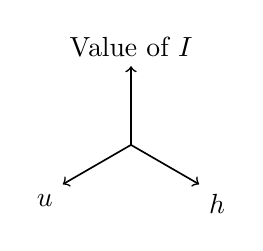
\begin{tikzpicture}
    \draw[->,semithick] (0,0) -- (0,1) node[above]{Value of $I$}; % z
    \draw[->,semithick] (0,0) -- +(-30:1) node[below right]{$h$}; % x
    \draw[->,semithick] (0,0) -- +(210:1) node[below left]{$u$}; % y
  \end{tikzpicture}
  \caption{Orientation of the axes used throughout the 3d-plots}
  \label{fig:orientation-of-axes}
\end{figure}

To plot $u$ and $h$ we need to know their respective ranges as well. This is noted in the caption of the whole figure. For example, in figure \ref{fig:two-points-all-the-same}, the values for $u$ are in $[9.5, 10.5]$ and the values for $h$ in $[-1,1]$.

Looking back at the caption of the subfigure, which had ``1/0.04'' in the latter part (subfigure \ref{subfig:fixing-p2-in-first-example}). This tells us the range of the values of $I$ (i.e. the ``$z$ axis''). To be precise, the firs part tells us that the maximal plotted value for the h component is 1, while the maximal $u$ component value is 0.04. A single number indicates a range between 0 and that number, while an explicit range indicates the given range (for an example, see \ref{subfig:example-with-range}, where the $h$ component plot range goes from 0.25 to 0.55, and the $u$ component from 0 to 0.03).

\section{Gaussian quadrature and distribution of support points}
\label{sec:results}

We implemented several scenarios and present the outcome of some of them using the support points one would use when doing a Gaussian quadrature. The $x$ values of these support points are summed up in this table:

\begin{table}[ht]
  \renewcommand\arraystretch{1.5}
  \centering
  \begin{tabular}[ht]{cl}
    Order & $x$-coordinates \\
    \hline
    2 & $\frac{1}{2}-\frac{1}{6}\cdot \sqrt{3}, \frac{1}{2}+\frac{1}{6}\cdot \sqrt{3}$ \\
    3 & $-\frac{1}{10}\cdot \sqrt{15}+\frac{1}{2} , 0.5, \frac{1}{10}\cdot \sqrt{15}+\frac{1}{2}$ \\
    \hline 
  \end{tabular}
  \caption{$x$-coordinates of support points for Gauss-Quadrature}
  \label{tab:x-coordinates-gauss-quadrature}
\end{table}

\subsection{Setting all support points to the same value}
\label{sec:setting-all-support-points-to-the-same-value}

First we set all support points to one single value ensuring homogenous height and impulse. Then, we tackle each point individually and let it's values range over a certain domain.

\begin{figure}[ht]
  \centering
  \subfigure[$p_1$: 1/0.04]{
    \includegraphics[scale=\zoomfactor]{2_equal_10_0/1_h.png} 
    \includegraphics[scale=\zoomfactor]{2_equal_10_0/1_u.png}
  }
  \subfigure[$p_2$: 1/0.04]{
    \label{subfig:fixing-p2-in-first-example}
    \includegraphics[scale=\zoomfactor]{2_equal_10_0/2_h.png} 
    \includegraphics[scale=\zoomfactor]{2_equal_10_0/2_u.png}
  }
  \subfigure[$P_1$: 1 / 0.04]{
    \includegraphics[scale=\zoomfactor]{2_equal_10_0/3_h.png} 
    \includegraphics[scale=\zoomfactor]{2_equal_10_0/3_u.png}
  }
  \subfigure[$P_2$: 1 / 0.04]{
    \includegraphics[scale=\zoomfactor]{2_equal_10_0/4_h.png} 
    \includegraphics[scale=\zoomfactor]{2_equal_10_0/4_u.png} 
  }
  \caption{Two points for each triangle. All support points have height 10 and impulse 0. $h$ ranges from 9.5 to 10.5, $u$ from -1 to 1.}
  \label{fig:two-points-all-the-same}
\end{figure}

Figure \ref{fig:two-points-all-the-same} shows the case for two points on each adjacent edge. The sub-figures are interpreted the following way: Each subfigure shows what happens if we fix all but one specific support point. For example, subfigure \ref{subfig:fixing-p2-in-first-example} shows what happens if we fix all support points except $p_2$ (containing the variables $h_2$ and $u_2$) and let range $h_2$ from 9.5 to 10.5 and $u_2$ from -1 to 1. The left part of subfigure \ref{subfig:fixing-p2-in-first-example} shows the error in the $h$-component, while the right half depicts the error in the $u$ component.

As you can see, the error for the $h$ component ranges up to 1, while the error in the $u$-component is probably negligible (namely about 0.04).

Of course it would be interesting to inspect the same thing for more support points along each edge. So we did for three support points along each edge. You can see the results in figure \ref{fig:three-points-equal}. Please note that the structure of the error plots seems to be the same all over. However, the error ranges vary slightly. For example, varying $P_2$ instead of $P_1$ (when using three points) results in different error levels (see figure \ref{subfig:3-points-ranging-P2} resp. \ref{subfig:3-points-ranging-P1}).

\begin{figure}[ht]
  \centering
  \subfigure[$p_1$: 0.8 / 0.03]{
    \label{subfig:3-points-equal-p1}
    \includegraphics[scale=\zoomfactor]{3_equal/1_h.png} 
    \includegraphics[scale=\zoomfactor]{3_equal/1_u.png} 
  }
  \subfigure[$p_2$: 1.2 / 0.05]{
    \includegraphics[scale=\zoomfactor]{3_equal/2_h.png} 
    \includegraphics[scale=\zoomfactor]{3_equal/2_u.png} 
  }
  \subfigure[$p_3$: 0.8 / 0.03]{
    \includegraphics[scale=\zoomfactor]{3_equal/3_h.png} 
    \includegraphics[scale=\zoomfactor]{3_equal/3_u.png} 
  }
  \subfigure[$P_1$: 0.8 / 0.03]{
    \label{subfig:3-points-ranging-P1}
    \includegraphics[scale=\zoomfactor]{3_equal/4_h.png} 
    \includegraphics[scale=\zoomfactor]{3_equal/4_u.png} 
  }
  \subfigure[$P_2$: 1.2 / 0.05]{
    \label{subfig:3-points-ranging-P2}
    \includegraphics[scale=\zoomfactor]{3_equal/5_h.png} 
    \includegraphics[scale=\zoomfactor]{3_equal/5_u.png} 
  }
  \subfigure[$P_3$: 0.8 / 0.03]{
    \includegraphics[scale=\zoomfactor]{3_equal/6_h.png} 
    \includegraphics[scale=\zoomfactor]{3_equal/6_u.png} 
  }
  \caption{Three points for each triangle. Points have height 10, impulse 0.}
  \label{fig:three-points-equal}
\end{figure}

\subsection{One point variation}
\label{sec:one-point-variation}

\subsubsection{Decreasing the height of $p_1$}
\label{sec:decreasing-height-p1}

Now we alter the previously described experiment in one detail. We fix all points as before, but we alter \emph{one} single point slightly. We do this in order to find out if specific points might have more impact than others.

We start off by using three points per edge, setting each point to $
\begin{pmatrix}
  10 \\ 0
\end{pmatrix}$ except $p_1$ wich is set to $
\begin{pmatrix}
  9 \\ 0
\end{pmatrix}
$ (i.e. we decrease the height-component of $p_1$).

\begin{figure}[ht]
  \centering
  \subfigure[$p_1$: 0.8 / 0.03]{
    \label{subfig:3-points-h1--equal-p1}
    \includegraphics[scale=\zoomfactor]{3_equal_h1-/1_h.png} 
    \includegraphics[scale=\zoomfactor]{3_equal_h1-/1_u.png} 
  }
  \subfigure[$p_2$: 1.6 / 0.1]{
    \includegraphics[scale=\zoomfactor]{3_equal_h1-/2_h.png} 
    \includegraphics[scale=\zoomfactor]{3_equal_h1-/2_u.png} 
  }
  \subfigure[$p_3$: 0.5 / 0.04]{
    \includegraphics[scale=\zoomfactor]{3_equal_h1-/3_h.png} 
    \includegraphics[scale=\zoomfactor]{3_equal_h1-/3_u.png} 
  }
  \subfigure[$P_1$: 1.1 / 0.03]{
    \label{subfig:3-points-h1--ranging-P1}
    \includegraphics[scale=\zoomfactor]{3_equal_h1-/4_h.png} 
    \includegraphics[scale=\zoomfactor]{3_equal_h1-/4_u.png} 
  }
  \subfigure[$P_2$: 1.3 / 0.05]{
    \label{subfig:3-points-h1--ranging-P2}
    \includegraphics[scale=\zoomfactor]{3_equal_h1-/5_h.png} 
    \includegraphics[scale=\zoomfactor]{3_equal_h1-/5_u.png} 
  }
  \subfigure[$P_3$: {$[0.25,0.55]$} /  0.03]{
    \includegraphics[scale=\zoomfactor]{3_equal_h1-/6_h.png} 
    \includegraphics[scale=\zoomfactor]{3_equal_h1-/6_u.png} 
  }
  \caption{Three points for each triangle. All points except $p_1$ have height 10, impulse 0. Point $p_1$ is set to $(9,0)$.}
  \label{fig:three-points-h1-}
\end{figure}

You see the results of this experiment in figure \ref{fig:three-points-h1-}. Please note that figure \ref{subfig:3-points-h1--equal-p1} and \ref{subfig:3-points-equal-p1} depict exactly the same thing, since $p_1$ is the only point we changed to differ from all the other points.

Comparing figure \ref{fig:three-points-equal} and \ref{fig:three-points-h1-} it's worth noting that especially the plots for $p_2$, $p_3$ and -- surprisingly -- $P_3$ differ strongly. Additionally, it can be seen that the structure differs as well as the range of the error.

\subsubsection{Decreasing the impulse of $p_1$}
\label{sec:decreasing-impulse-p1}

While we changed the height in subsection \ref{sec:decreasing-height-p1}, we are now going to change the impulse. The results are shown in figure \ref{fig:three-points-u1-}

\begin{figure}[ht]
  \centering
  \subfigure[$p_1$: 0.8 / 0.03]{
    \includegraphics[scale=\zoomfactor]{3_equal_u1-/1_h.png} 
    \includegraphics[scale=\zoomfactor]{3_equal_u1-/1_u.png} 
  }
  \subfigure[$p_2$: 2.5 / 0.07]{
    \includegraphics[scale=\zoomfactor]{3_equal_u1-/2_h.png} 
    \includegraphics[scale=\zoomfactor]{3_equal_u1-/2_u.png} 
  }
  \subfigure[$p_3$: 1 / 0.03]{
    \includegraphics[scale=\zoomfactor]{3_equal_u1-/3_h.png} 
    \includegraphics[scale=\zoomfactor]{3_equal_u1-/3_u.png} 
  }
  \subfigure[$P_1$: {$[0.7, 1.5]$} / 0.03]{
    \includegraphics[scale=\zoomfactor]{3_equal_u1-/4_h.png} 
    \includegraphics[scale=\zoomfactor]{3_equal_u1-/4_u.png} 
  }
  \subfigure[$P_2$: 1 / 0.05]{
    \includegraphics[scale=\zoomfactor]{3_equal_u1-/5_h.png} 
    \includegraphics[scale=\zoomfactor]{3_equal_u1-/5_u.png} 
  }
  \subfigure[$P_3$: {$[0.45,0.65]$} /  0.03]{
    \label{subfig:example-with-range}
    \includegraphics[scale=\zoomfactor]{3_equal_u1-/6_h.png} 
    \includegraphics[scale=\zoomfactor]{3_equal_u1-/6_u.png} 
  }
  \caption{Three points for each triangle. All points except $p_1$ have height 10, impulse 0. Point $p_1$ is set to $(10,-1)$.}
  \label{fig:three-points-u1-}
\end{figure}

Again, the plots for $p_2$, $p_3$ and $P_6$ differ in structure extremely from those depicted in figure \ref{fig:three-points-equal}. In this context it would be interesting to know what happens with the plot of the height of $p_3$ if the impulse grows bigger than 1, since it looks like the error goes down at the left end. We created a plot that shows the behaviour of the error when $p_3$ ranges. It is depicted in figure \ref{fig:examining-p3-three-points}. As you can see, it was just an ``optical illustion'' due to the particular ranges we chose for the $h$- and $u$- component. The error grows towards the borders.

\begin{figure}[ht]
  \centering
  \includegraphics[scale=\autozoomfactor]{3_fix_p1_u_larger2/3_h.png}
  \includegraphics[scale=\autozoomfactor]{3_fix_p1_u_larger2/3_u.png}
  \caption{Examining $p_3$ for three points, all having value $(10,0)$ except $p_1$ having $(10,-1)$. The error in the $h$-component grows up to 15, while the error in $u$ reaches a maximum of 0.55 ($u$ ranging in $[-2,2]$, $h$ ranging in $[6,14]$)}
  \label{fig:examining-p3-three-points}
\end{figure}

 Moreover, the error for $p_2$ increases to 2.5.

\subsubsection{Decreasing the height of $p_2$}
\label{sec:decreasing-height-p2}

Now we are going to examine if it makes a difference if we decrease the height of another point, namely $p_2$. We show the results in figure \ref{fig:three-points-h2-}. In this case, in particular the graphs for points $p_1$ and $p_3$ catch one's eye.

\begin{figure}[ht]
  \centering
  \subfigure[$p_1$: {$[0.4, 1.4]$} / 0.1]{
    \includegraphics[scale=\zoomfactor]{3_equal_h2-/1_h.png} 
    \includegraphics[scale=\zoomfactor]{3_equal_h2-/1_u.png} 
  }
  \subfigure[$p_2$: 1.2 / 0.05]{
    \includegraphics[scale=\zoomfactor]{3_equal_h2-/2_h.png} 
    \includegraphics[scale=\zoomfactor]{3_equal_h2-/2_u.png} 
  }
  \subfigure[$p_3$: {$[0.6, 1.4]$} / 0.1]{
    \includegraphics[scale=\zoomfactor]{3_equal_h2-/3_h.png} 
    \includegraphics[scale=\zoomfactor]{3_equal_h2-/3_u.png} 
  }
  \subfigure[$P_1$: {$[0.5, 1]$} / 0.03]{
    \includegraphics[scale=\zoomfactor]{3_equal_h2-/4_h.png} 
    \includegraphics[scale=\zoomfactor]{3_equal_h2-/4_u.png} 
  }
  \subfigure[$P_2$: {$[0.6, 1.6]$} / 0.05]{
    \includegraphics[scale=\zoomfactor]{3_equal_h2-/5_h.png} 
    \includegraphics[scale=\zoomfactor]{3_equal_h2-/5_u.png} 
  }
  \subfigure[$P_3$: {$[0.6, 1]$} /  0.03]{
    \includegraphics[scale=\zoomfactor]{3_equal_h2-/6_h.png} 
    \includegraphics[scale=\zoomfactor]{3_equal_h2-/6_u.png} 
  }
  \caption{Three points for each triangle. All points except $p_2$ have height 10, impulse 0. Point $p_2$ is set to $(9,0)$.}
  \label{fig:three-points-h2-}
\end{figure}

\subsubsection{Decreasing the impulse of $p_2$}
\label{sec:decreasing-impulse-of-p2}

Decreasing the impulse of point $p_2$ results in the plots depicted in figure \ref{fig:three-points-u2-}. In particular, the graphs for $p_1$ and $p_3$ show significant structural differences.

\begin{figure}[ht]
  \centering
  \subfigure[$p_1$: {$[0.6, 2.5]$} / 0.06]{
    \includegraphics[scale=\zoomfactor]{3_equal_u2-/1_h.png} 
    \includegraphics[scale=\zoomfactor]{3_equal_u2-/1_u.png} 
  }
  \subfigure[$p_2$: 1.2 / 0.05]{
    \includegraphics[scale=\zoomfactor]{3_equal_u2-/2_h.png} 
    \includegraphics[scale=\zoomfactor]{3_equal_u2-/2_u.png} 
  }
  \subfigure[$p_3$: {$[0.5, 2.7]$} / 0.06]{
    \includegraphics[scale=\zoomfactor]{3_equal_u2-/3_h.png} 
    \includegraphics[scale=\zoomfactor]{3_equal_u2-/3_u.png} 
  }
  \subfigure[$P_1$: {$[1, 1.4]$} / 0.03]{
    \includegraphics[scale=\zoomfactor]{3_equal_u2-/4_h.png} 
    \includegraphics[scale=\zoomfactor]{3_equal_u2-/4_u.png} 
  }
  \subfigure[$P_2$: {$[1.2, 2.2]$} / 0.05]{
    \includegraphics[scale=\zoomfactor]{3_equal_u2-/5_h.png} 
    \includegraphics[scale=\zoomfactor]{3_equal_u2-/5_u.png} 
  }
  \subfigure[$P_3$: {$[1, 1.4]$} /  0.03]{
    \includegraphics[scale=\zoomfactor]{3_equal_u2-/6_h.png} 
    \includegraphics[scale=\zoomfactor]{3_equal_u2-/6_u.png} 
  }
  \caption{Three points for each triangle. All points except $p_2$ have height 10, impulse 0. Point $p_2$ is set to $(10,-1)$.}
  \label{fig:three-points-u2-}
\end{figure}

\subsection{Random values}
\label{sec:random-values}

And now for something completely different. Up to now, we assigned specific values to the points and looked what happened. But it might be interesting as well what happens if we supply random values to the points.

\subsubsection{Two random points}
\label{sec:two-random-points}

Let's start out with two random points. We see the results of random assignment of values in figure \ref{fig:two-points-random}. As you can see, there are heavy structural differences. The maximum error concerning the height is about 6.

\begin{figure}[ht]
  \centering
  \subfigure[$p_1$: {$[1,3]$} / 0.1]{
    \includegraphics[scale=\zoomfactor]{2_random/1_h.png} 
    \includegraphics[scale=\zoomfactor]{2_random/1_u.png}
  }
  \subfigure[$p_2$: {$[1, 2.6]$} / 0.16]{
    \includegraphics[scale=\zoomfactor]{2_random/2_h.png} 
    \includegraphics[scale=\zoomfactor]{2_random/2_u.png}
  }  
  \subfigure[$P_1$: 4 / 0.2]{
    \includegraphics[scale=\zoomfactor]{2_random/3_h.png} 
    \includegraphics[scale=\zoomfactor]{2_random/3_u.png}
  }
  \subfigure[$P_2$: {$[1,6]$} / 0.2]{
    \includegraphics[scale=\zoomfactor]{2_random/4_h.png} 
    \includegraphics[scale=\zoomfactor]{2_random/4_u.png} 
  }
  \caption{Two points for each triangle. Values for the points are: $u_1^R = -0.082$, $h_1^R = 9.4$, $u_2^R = -0.45$, $h_2^R = 10.33$, $u_1^L = -1.32$, $h_1^L = 9.45$, $u_2^L = -0.75$, $h_2^L = 10.72$. }
  \label{fig:two-points-random}
\end{figure}

\subsubsection{Three random points}
\label{sec:three-random-points}

Same game for three random points is shown in figure \ref{fig:three-points-random}. As you can see, it differs strongly from figure \ref{fig:three-points-equal}, where we set all points to the same value.

\begin{figure}[ht]
  \centering
  \subfigure[$p_1$: {$[1, 2.2]$} / 0.12]{
    \includegraphics[scale=\zoomfactor]{3_random/1_h.png} 
    \includegraphics[scale=\zoomfactor]{3_random/1_u.png} 
  }
  \subfigure[$p_2$: {$[1, 3]$} / 0.12]{
    \includegraphics[scale=\zoomfactor]{3_random/2_h.png} 
    \includegraphics[scale=\zoomfactor]{3_random/2_u.png} 
  }
  \subfigure[$p_3$: {$[1.2, 1.7]$} / {$[0.05, 0.11]$}]{
    \includegraphics[scale=\zoomfactor]{3_random/3_h.png} 
    \includegraphics[scale=\zoomfactor]{3_random/3_u.png} 
  }
  \subfigure[$P_1$: {$[1, 4.5]$} / 0.18]{
    \includegraphics[scale=\zoomfactor]{3_random/4_h.png} 
    \includegraphics[scale=\zoomfactor]{3_random/4_u.png} 
  }
  \subfigure[$P_2$: {$[1, 4.5]$} / {$[0.04, 0.16]$}]{
    \includegraphics[scale=\zoomfactor]{3_random/5_h.png} 
    \includegraphics[scale=\zoomfactor]{3_random/5_u.png} 
  }
  \subfigure[$P_3$: {$[1.5, 5]$} /  {$[0.06, 0.12]$}]{
    \includegraphics[scale=\zoomfactor]{3_random/6_h.png} 
    \includegraphics[scale=\zoomfactor]{3_random/6_u.png} 
  }
  \caption{Three random points for each triangle}
  \label{fig:three-points-random}
\end{figure}

\clearpage

\section{Equidistant distribution of support points}
\label{sec:equidistant-distribution-of-support-points}

When one considers the figures depicted in section \ref{sec:results}, it seems convenient to assume that the error grows if the values for $h$ and $u$ get ``more exotic'' (i.e. if they diverge more from the average).

One suspicion why this is the case was because of the fact that the polynomials $N(x)$ and $N'(x)$ might diverge towards the borders of $[0,1]$.

So, we chose the support points equidistant over the interval $[0,1]$ and conducted some experiments. When we choose the support points equidistant over this interval, 0 and 1 are surely support points and we can be sure that $N(x)$ and $N'(x)$ coincide at the values 0 and 1 (i.e. $N(0)=N'(0)$ and $N(1)=N'(1)$).

In this section, we show some results that were obtained by choosing the support points equidistant along the edge.

\subsection{Three fixed support points}
\label{sec:equidistant-three-fixed}

We started as in section \ref{sec:setting-all-support-points-to-the-same-value} and set all support points to $
\begin{pmatrix}
  10 \\ 0
\end{pmatrix}$. You can see the resulting plots in figure \ref{fig:three-equidistant-all-fixed}. Interestingly, these plots -- at least somewhat -- look like the ones depicted in figure \ref{fig:three-points-equal}, where we considered the same situation for Gauss-Quadrature support points. Even the range of the error is not very different.

\input{3_equidist_fix/figure.tex}

\section{Conclusions from the things seen}
\label{sec:conslusions}

What all plots have in common is the fact that it looks as if towards the borders the error grows. Trying to derive an exact statement of how large the error is depending upon the support point values seems a bit witless since there are too many variables that interact with each other.

\subsection{Making this interactive}
\label{sec:making-the-whole-thing-interactive}

As you might know, Maple supports kind of ``dynamic plotting''. That is, you get a window containing one slider for each variable in a mathematical expression. You can then plot this expression

\end{comment}

\end{document}
